\input{mmd-beamer-header}
\def\mytitle{What is MultiMarkdown?}
\def\subtitle{And why should you care?}
\def\myauthor{Fletcher T. Penney}
\def\affiliation{http:/\slash fletcherpenney.net\slash multimarkdown\slash }
\def\mycopyright{2009-2011 Fletcher T. Penney.  \\
This work is licensed under a Creative Commons License.  \\
http:/\slash creativecommons.org\slash licenses\slash by-sa\slash 2.5\slash }
\def\latexmode{beamer}
\input{mmd-natbib-plain}
\def\theme{keynote-gradient}
\input{mmd-beamer-begin-doc}
\begin{frame}

\frametitle{MultiMarkdown is a derivative of Markdown}
\label{multimarkdownisaderivativeofmarkdown}

\href{http://daringfireball.net/projects/markdown/}{Markdown}\footnote{\href{http://daringfireball.net/projects/markdown/}{http:/\slash daringfireball.net\slash projects\slash markdown\slash }} is a program and a
syntax by John Gruber that allows you to easily convert plain text into HTML
suitable for using on a web page.

\end{frame}

\begin{frame}[fragile]

\frametitle{The old way was complicated}
\label{theoldwaywascomplicated}

\begin{verbatim}
<p>In order to create valid 
<a href="http://en.wikipedia.org/wiki/HTML">HTML</a>, you 
need properly coded syntax that can be cumbersome for 
&#8220;non-programmers&#8221; to write. Sometimes, you
just want to easily make certain words <strong>bold
</strong>, and certain words <em>italicized</em> without
having to remember the syntax. Additionally, for example,
creating lists:</p>

<ul>
<li>should be easy</li>
<li>should not involve programming</li>
</ul>
\end{verbatim}


\end{frame}

\begin{frame}[fragile]

\frametitle{The new way is easier}
\label{thenewwayiseasier}

\begin{verbatim}
In order to create valid [HTML], you need properly
coded syntax that can be cumbersome for 
"non-programmers" to write. Sometimes, you just want
to easily make certain words **bold**, and certain 
words *italicized* without having to remember the 
syntax. Additionally, for example, creating lists:

* should be easy
* should not involve programming

[HTML]: http://en.wikipedia.org/wiki/HTML
\end{verbatim}


\end{frame}

\begin{frame}

\frametitle{Markdown is designed for people}
\label{markdownisdesignedforpeople}

The overriding design goal for Markdown's formatting syntax is to make it as
readable as possible. The idea is that a Markdown-formatted document should be
publishable as-is, as plain text, without looking like it's been marked up
with tags or formatting instructions. While Markdown's syntax has been
influenced by several existing text-to-HTML filters, the single biggest source
of inspiration for Markdown's syntax is the format of plain text email.
~\citep{Gruber}

\end{frame}

\begin{frame}

\frametitle{But Markdown wasn't complete}
\label{butmarkdownwasntcomplete}

I, and others, loved the spirit and elegance of Markdown, but felt it was
still missing a few features that each of us considered were essential.
Several variations on Markdown arose to meet the needs of these other
programmers.

\end{frame}

\begin{frame}

\frametitle{MultiMarkdown adds several new features}
\label{multimarkdownaddsseveralnewfeatures}

\begin{itemize}
\item footnotes

\item tables

\item citations and bibliography

\item image attributes

\item metadata

\item internal cross-references

\item math support

\item glossary entries

\item definition lists

\item and more{\ldots}

\end{itemize}

\end{frame}

\begin{frame}

\frametitle{MMD also adds something else{\ldots}}
\label{mmdalsoaddssomethingelse}

\begin{itemize}
\item Outside of the actual syntax, MMD supports multiple output formats,
 including HTML, \href{http://en.wikipedia.org/wiki/LaTeX}{LaTeX}\footnote{\href{http://en.wikipedia.org/wiki/LaTeX}{http:/\slash en.wikipedia.org\slash wiki\slash LaTeX}},
 \href{http://en.wikipedia.org/wiki/OpenDocument}{OpenDocument}\footnote{\href{http://en.wikipedia.org/wiki/OpenDocument}{http:/\slash en.wikipedia.org\slash wiki\slash OpenDocument}}, and
 \href{http://en.wikipedia.org/wiki/OPML}{OPML}\footnote{\href{http://en.wikipedia.org/wiki/OPML}{http:/\slash en.wikipedia.org\slash wiki\slash OPML}}

\item This allows you to use the same markup language (MultiMarkdown) to create a
 high quality pdf (article, book, or presentation like this one) without any
 additional programming.

\item Most importantly, you don't have to know how this works, or even what it
 the LaTeX commands mean --- just have the software installed.

\end{itemize}

\end{frame}

\begin{frame}

\frametitle{So, one text file becomes multiple final documents}
\label{soonetextfilebecomesmultiplefinaldocuments}

\begin{figure}[htbp]
\centering
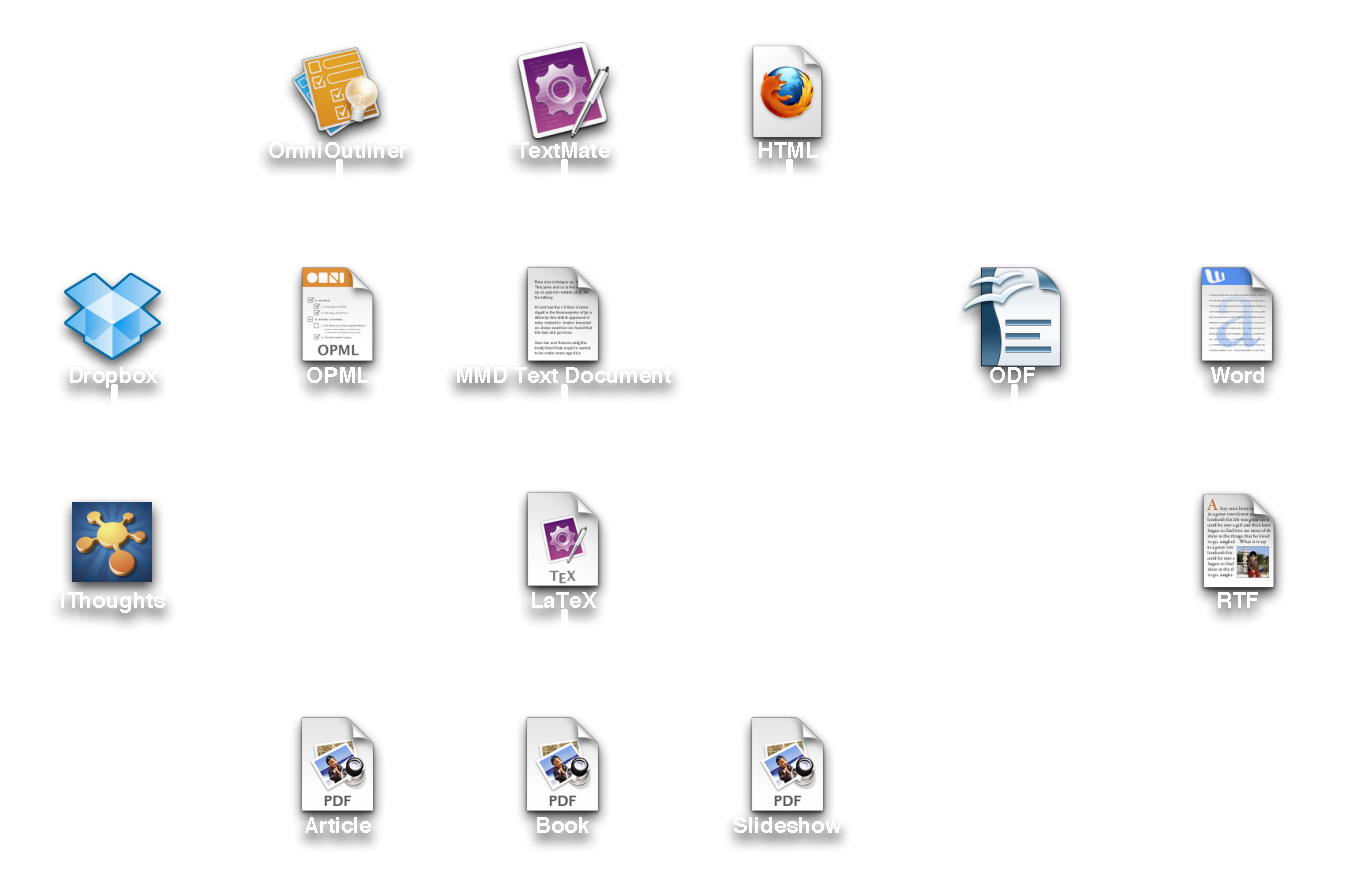
\includegraphics[keepaspectratio,width=\textwidth,height=0.75\textheight]{OPML-MMD-Map.pdf}
\caption{Example MultiMarkdown output formats}
\label{}
\end{figure}


\end{frame}

\begin{frame}

\frametitle{The goal is to separate content from formatting}
\label{thegoalistoseparatecontentfromformatting}

By focusing on the text content of your document, you can focus on the
creative, the scientific, the \emph{human}. Let your computer do what it is good at
--- the fairly boring job of making sure that margins are correct, that
paragraphs are properly separated, your footnotes are in order, and that your
tables line up --- regardless of the final format you want your document to
take.

\end{frame}

\begin{frame}[fragile]

\frametitle{MultiMarkdown and Mathematics}
\label{multimarkdownandmathematics}

Built into MultiMarkdown is support for mathematical equations. You write
using LaTeX syntax. When you output to HTML, you can use
\href{http://www.mathjax.org/}{MathJax}\footnote{\href{http://www.mathjax.org/}{http:/\slash www.mathjax.org\slash }} to properly display the math. If you output
to LaTeX, it is display automatically. There is not currently an approach to
display math using OpenDocument

\begin{verbatim}
\\[ {e}^{i\pi }+1=0 \\]
\end{verbatim}


becomes

\[ {e}^{i\pi }+1=0 \]

\end{frame}

\begin{frame}[fragile]

\frametitle{Images are just as easy}
\label{imagesarejustaseasy}

\begin{verbatim}
![Nautilus Star](Nautilus_Star.png)
\end{verbatim}


becomes{\ldots}

\end{frame}

\begin{frame}

\frametitle{Images are just as easy}
\label{imagesarejustaseasy}

\begin{figure}[htbp]
\centering
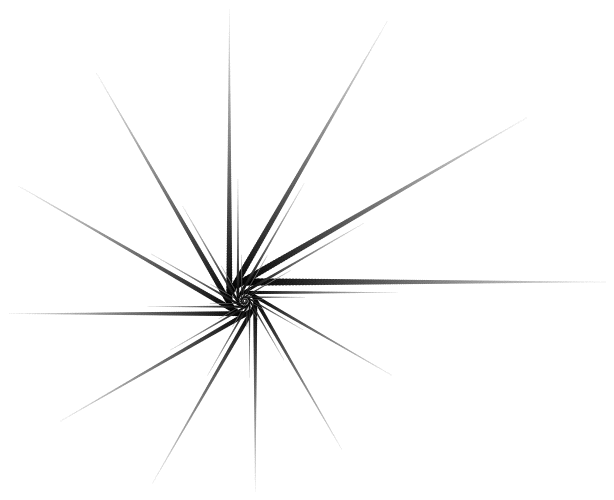
\includegraphics[keepaspectratio,width=\textwidth,height=0.75\textheight]{Nautilus_Star.png}
\caption{Nautilus Star}
\label{}
\end{figure}


\end{frame}

\begin{frame}

\frametitle{Support for a bibliography is also included}
\label{supportforabibliographyisalsoincluded}

\begin{itemize}
\item MultiMarkdown has support for \href{http://www.bibtex.org/}{BibTeX}\footnote{\href{http://www.bibtex.org/}{http:/\slash www.bibtex.org\slash }}, or
 for just including your own citations, so that you can back up your
 arguments.~\citep[p. 42]{fake}

\item The citation above links to the corresponding entry in the bibliography.

\end{itemize}

\end{frame}

\begin{frame}

\frametitle{Installation is easy}
\label{installationiseasy}

\begin{itemize}
\item Download the MultiMarkdown software --- there are installers for Mac OS X
 and Windows, and instructions for compiling in Linux.

\item If you want to use LaTeX, install a version appropriate for your operating
 system.

\item OpenDocument output doesn't require any special software, but will require
 an application capable of opening the document --- LibreOffice,
 OpenOffice.org (with the proper plug-in installed), etc.

\end{itemize}

\end{frame}

\begin{frame}

\frametitle{How do I create a MultiMarkdown document?}
\label{howdoicreateamultimarkdowndocument}

\begin{itemize}
\item A MultiMarkdown is simply a text document that is written in the
 MultiMarkdown syntax. You can use any text editor or application you like.
 If your editor supports fonts, italics, etc. then be sure to save as a plain
 text file (not a .doc, RTF, or other ``rich'' format).

\item Some applications include built-in support for MultiMarkdown in various
 ways. There's a \href{http://fletcher.github.com/markdown.tmbundle/}{bundle}\footnote{\href{http://fletcher.github.com/markdown.tmbundle/}{http:/\slash fletcher.github.com\slash markdown.tmbundle\slash }} for \href{http://macromates.com/}{TextMate}\footnote{\href{http://macromates.com/}{http:/\slash macromates.com\slash }}, and \href{http://www.literatureandlatte.com/scrivener.html}{Scrivener}\footnote{\href{http://www.literatureandlatte.com/scrivener.html}{http:/\slash www.literatureandlatte.com\slash scrivener.html}} includes
 MultiMarkdown support.

\end{itemize}

\end{frame}

\begin{frame}

\frametitle{Why should I mess with this LaTeX stuff?}
\label{whyshouldimesswiththislatexstuff}

MultiMarkdown's support for LaTeX is designed to automatically do the ``right''
thing in most situations for most people. But if you want to dig in and learn
more, you can customize MMD to create highly tailored documents that suit your
specific needs. If you want high quality typography, LaTeX is the way to go.

If you already know what LaTeX is, then MultiMarkdown allows you to create
documents without learning all of the complicated LaTeX commands and markup.

\end{frame}

\begin{frame}

\frametitle{How do I create a fancy PDF?}
\label{howdoicreateafancypdf}

If you're using LaTeX, and have the proper software installed it's easy:

\begin{enumerate}
\item Type \texttt{mmd2tex filename.txt}

\item Use \texttt{pdflatex}, \texttt{xelatex}, or your preferred tool to compile the LaTeX
 file into a pdf.

\item There is no step 3

\end{enumerate}

\end{frame}

\begin{frame}

\frametitle{Where to learn more}
\label{wheretolearnmore}

\begin{itemize}
\item \href{http://fletcherpenney.net/multimarkdown/}{http:/\slash fletcherpenney.net\slash multimarkdown\slash }

\item \href{http://groups.google.com/group/multimarkdown/}{http:/\slash groups.google.com\slash group\slash multimarkdown\slash }

\item \href{http://fletcher.github.com/MultiMarkdown-Gallery/}{http:/\slash fletcher.github.com\slash MultiMarkdown-Gallery\slash }

\end{itemize}

\end{frame}

\begin{frame}

\frametitle{By the way{\ldots}}
\label{bytheway}

This presentation was, of course, written in MultiMarkdown and processed by
typing \texttt{mmd2tex what\_is\_mmd.txt}.

It uses the \texttt{beamer} XSLT file, and the \texttt{keynote-gradient} beamer theme.

\end{frame}

\part{Bibliography}
\begin{frame}[allowframebreaks]
\frametitle{Bibliography}
\def\newblock{}
\begin{thebibliography}{0}
\bibitem{Gruber}
John Gruber. Daring Fireball: Markdown. [Cited January 2006]. Available from \href{http://daringfireball.net/projects/markdown/}{http:/\slash daringfireball.net\slash projects\slash markdown\slash }.


\bibitem{fake}
John Doe. \emph{A Totally Fake Book}. Vanity Press, 2006.


\end{thebibliography}
\end{frame}

\mode<all>
\input{mmd-beamer-footer}

\end{document}\mode*

